\documentclass[11pt,a4paper]{article}
\usepackage[T1]{fontenc}
\usepackage{lmodern}
\usepackage[latin1]{inputenc}
\usepackage{ngerman}
\usepackage{a4wide}
\usepackage[dvips]{graphicx}
\usepackage{float}
\restylefloat{figure}
\restylefloat{table}

\usepackage[
a4paper,
pdfauthor={ ACE Projekt Team },
pdftitle={ Projektplan },
pdfcreator={pdftex},
]{hyperref}

\usepackage{sectsty}
\allsectionsfont{\sffamily}

\usepackage{fancyheadings} 
\pagestyle{fancy} 
\lhead{\textsf{\textbf{ACE} \\ \small{a collaborative editor}}}
\chead{}
\rhead{
\includegraphics[height=0.875cm,width=3cm]{../../images/logo_BFH.eps}}
\lfoot{}
\cfoot{\textsf{\thepage}}
\rfoot{}
\setlength{\headrulewidth}{0.6pt}
\setlength{\footrulewidth}{0.6pt}
\setlength{\topmargin}{-50pt}
\addtolength{\headheight}{50pt}

\usepackage{colortbl}

\newcommand{\headercol}[2]{\multicolumn{1}{|>{\bfseries\columncolor[gray]{0.82}}p{#1}|}{\textsf{#2}}}
\newcommand{\ace}[0]{\emph{ACE }}



\begin{document}

\begin{titlepage}
\thispagestyle{empty}
  \includegraphics[height=1.5in]{../../images/pix.eps}

  \begin{center}

    {\fontsize{40}{45} \textbf{\textsf{ACE}}} \\
    \textsf{a collaborative editor} \\
        
    \vspace{36pt}
        
    {\huge{\textbf{\textsf{Report Evaluation Network}}}} \\

    \vspace{36pt}

	\textsf{Berne University of Applied Sciences} \\
    \textsf{School of Engineering and Information Technology} \\
    
  \end{center}

  \vfill
  
  \begin{tabular}{ll}
   \hline

   \\

   \multicolumn{1}{>{\bfseries}p{1.5in}}{\textsf{Date:}} &
   \multicolumn{1}{>{}p{4.3in}}{\textsf{14.06.2005}}          \\
   
   \\
   
   \multicolumn{1}{>{\bfseries}p{1.5in}}{\textsf{Version:}}     &   
   \multicolumn{1}{>{}p{4.3in}}{\textsf{0.6}}                 \\

   \\
   
   \multicolumn{1}{>{\bfseries}p{1.5in}}{\textsf{Projectteam:}}                 &
   \multicolumn{1}{>{}p{4.3in}}{\textsf{Mark Bigler (biglm2@hta-bi.bfh.ch)}}  \\
   \multicolumn{1}{>{\bfseries}p{1.5in}}{}                                      &
   \multicolumn{1}{>{}p{4.3in}}{\textsf{Simon R�ss (rasss@hta-bi.bfh.ch)}}    \\
   \multicolumn{1}{>{\bfseries}p{1.5in}}{}                                      &
   \multicolumn{1}{>{}p{4.3in}}{\textsf{Lukas Zbinden (zbinl@hta-bi.bfh.ch)}} \\   
   
   \\
   
   \multicolumn{1}{>{\bfseries}p{1.5in}}{\textsf{Receivers:}}                       &
   \multicolumn{1}{>{}p{4.3in}}{\textsf{Jean-Paul Dubois (doj@hta-bi.bfh.ch)}}       \\
   \multicolumn{1}{>{\bfseries}p{1.5in}}{}                                          &
   \multicolumn{1}{>{}p{4.3in}}{\textsf{Claude Fuhrer (frc@hta-bi.bfh.ch)}}       \\

   \\
   
   \multicolumn{1}{>{\bfseries}p{1.5in}}{\textsf{Location:}}               &   
   \multicolumn{1}{>{}p{4.3in}}{\textsf{Subversion Repository}} \\

   \\  
   
   \hline
  \end{tabular}

\end{titlepage}

\newpage

\tableofcontents
\newpage
\listoftables
\listoffigures
\newpage

\section*{Versionskontrolle}

\begin{table}[!h]
 \begin{tabular}{|l|l|l|l|}
  \hline
  \headercol{0.6in}{Version}         & 
  \headercol{0.8in}{Datum}           &
  \headercol{1.2in}{Verantwortlich}  & 
  \headercol{2.8in}{Bemerkungen}     \\
  \hline
  0.1         & 15.03.2005  & zbinl           &  Erste Version \\
  0.2         & 16.03.2005  & Projektteam     &  �berarbeitung \\
  0.3         & 05.04.2005  & Projektteam     &  �berarbeitung vor Abgabe \\
  \hline
 \end{tabular}
 \caption{Versionskontrolle}
 \label{Versionskontrolle}
\end{table}

\begin{table}[!h]
 \begin{tabular}{|l|l|l|l|l|}
  \hline
  \headercol{0.9in}{}            & 
  \headercol{0.9in}{Stelle}      & 
  \headercol{0.8in}{Datum}       & 
  \headercol{0.6in}{Visum}       & 
  \headercol{2.0in}{Bemerkungen} \\
  \hline
  \textbf{Freigegeben}   & Projektteam &       &       &             \\
  \hline
  \textbf{Genehmigt}     &             &       &       &             \\
  \hline
 \end{tabular}
 \caption{Pr�fung/Genehmigung}
 \label{Pr�fung/Genehmigung}
\end{table}

\newpage


\section{Einleitung}
\subsection{Zweck des Dokumentes}
Der Projektplan enth�lt die Planung und Organisation des gesamten Projekts und erg�nzt das Projekthandbuch als Handlungsgrundlage. Der Projektplan wird fortlaufend nachgef�hrt und verfeinert.


\section{Projektorganisation}


\section{Projektablauf}
Der Projektablauf beschreibt die Ergebnisstruktur des \ace Projektes und darauf aufbauend die ablaufoganisatorischen Gegebenheiten.


\subsection{Ergebnisstruktur}
Alle Ergebnisse, die zum jeweiligen Planungsstand bekannt sind, werden identifiziert und in ihrer Abh�ngigkeit (Struktur) untereinander festgelegt. Dieser Abschnitt enth�lt sowohl die als Vertragsbestandteil festgelegten Ergebnisse als auch die projekinternen Ergebnisse.

\begin{figure}[H]
 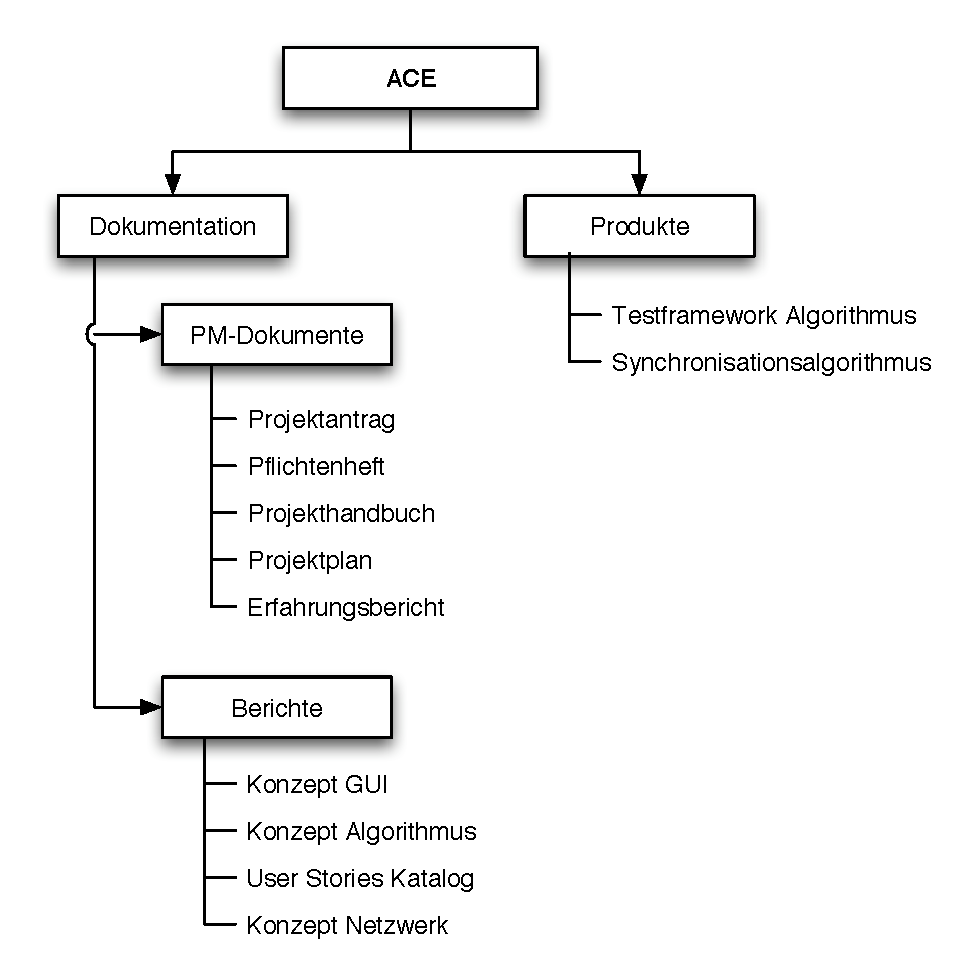
\includegraphics[width=5.5in,height=5.5in]{../../images/ergebnisstrukturplan.eps}
 \caption{Ergebnisstrukturplan}
 \label{Ergebnisstrukturplan}
\end{figure}


\subsection{Workpackages}

\begin{table}[H]
 \begin{tabular}{|l|l|l|l|}
  \hline
    \multicolumn{3}{|>{\columncolor[gray]{0.82}}p{5.85in}|}{\bfseries{\textsf{Work Package: Infrastruktur}}} \\
  \hline
    \multicolumn{1}{|p{1in}|}{\bfseries{\textsf{Autor}}} &
    \multicolumn{2}{|p{4.5in}|}{Projektteam} \\
  \hline
    \multicolumn{1}{|p{1in}|}{\bfseries{\textsf{Datum}}} &
    \multicolumn{2}{|p{4.5in}|}{29.3.2005} \\
  \hline
    \multicolumn{1}{|p{1in}|}{\bfseries{\textsf{Input}}} &
    \multicolumn{2}{|p{4.5in}|}{} \\
  \hline
    \multicolumn{1}{|p{1in}|}{\bfseries{\textsf{Output}}} &
    \multicolumn{2}{|p{4.5in}|}{Entwicklungsumgebung} \\
    \multicolumn{1}{|p{1in}|}{} &
    \multicolumn{2}{|p{4.5in}|}{Projekt Server} \\
    \multicolumn{1}{|p{1in}|}{} &
    \multicolumn{2}{|p{4.5in}|}{Projekt Website} \\
  \hline
   \multicolumn{1}{|p{1in}|}{\bfseries{\textsf{Skills}}} &
   \multicolumn{2}{|p{4.5in}|}{Installationserfahrung Subversion, Trac, Kalender} \\
  \hline
   \multicolumn{1}{|p{1in}|}{\bfseries{\textsf{Resources}}} &
   \multicolumn{2}{|p{4.5in}|}{Hardware und Software f�r Arbeitspl�tze} \\
   \multicolumn{1}{|p{1in}|}{} &
   \multicolumn{2}{|p{4.5in}|}{Zugriff Projektserver} \\
    
  \hline \hline
    \multicolumn{1}{|>{\columncolor[gray]{0.82}}p{1in}|}{} &
    \multicolumn{1}{|>{\columncolor[gray]{0.82}}p{3.5in}|}{\bfseries{\textsf{Beschreibung}}} &
    \multicolumn{1}{|>{\columncolor[gray]{0.82}}p{1in}|}{\bfseries{\textsf{Aufwand}}} \\
  \hline
    \multicolumn{1}{|p{1in}|}{\bfseries{\textsf{Aktivit�ten}}} &
    \multicolumn{1}{|p{3.5in}|}{PC installieren} &
    \multicolumn{1}{|p{1in}|}{2 Tage} \\
    \multicolumn{1}{|p{1in}|}{} &
    \multicolumn{1}{|p{3.5in}|}{Projekt Server installieren (Subversion, Trac, Kalender)} &
    \multicolumn{1}{|p{1in}|}{1 Tag} \\
    \multicolumn{1}{|p{1in}|}{} &
    \multicolumn{1}{|p{3.5in}|}{Projekt Website einrichten} &
    \multicolumn{1}{|p{1in}|}{1 Tag} \\    
  \hline
    \multicolumn{1}{|p{1in}|}{\bfseries{\textsf{QA}}} &
    \multicolumn{1}{|p{3.5in}|}{} &
    \multicolumn{1}{|p{1in}|}{} \\
  \hline \hline
    \multicolumn{1}{|p{1in}|}{\bfseries{\textsf{Total}}} &
    \multicolumn{1}{|p{3.5in}|}{} &
    \multicolumn{1}{|p{1in}|}{4 Tage} \\
  \hline
 \end{tabular}
 \caption{Workpackage Infrastruktur}
 \label{Workpackage Infrastruktur}
\end{table}


\begin{table}[H]
 \begin{tabular}{|l|l|l|l|}
  \hline
    \multicolumn{3}{|>{\columncolor[gray]{0.82}}p{5.85in}|}{\bfseries{\textsf{Work Package: Projektantrag}}} \\
  \hline
    \multicolumn{1}{|p{1in}|}{\bfseries{\textsf{Autor}}} &
    \multicolumn{2}{|p{4.5in}|}{Simon R�ss} \\
  \hline
    \multicolumn{1}{|p{1in}|}{\bfseries{\textsf{Datum}}} &
    \multicolumn{2}{|p{4.5in}|}{5.4.2005} \\
  \hline
    \multicolumn{1}{|p{1in}|}{\bfseries{\textsf{Input}}} &
    \multicolumn{2}{|p{4.5in}|}{keiner} \\
  \hline \hline
    \multicolumn{1}{|>{\columncolor[gray]{0.82}}p{1in}|}{} &
    \multicolumn{1}{|>{\columncolor[gray]{0.82}}p{3.5in}|}{\bfseries{\textsf{Beschreibung}}} &
    \multicolumn{1}{|>{\columncolor[gray]{0.82}}p{1in}|}{\bfseries{\textsf{Aufwand}}} \\
  \hline
    \multicolumn{1}{|p{1in}|}{\bfseries{\textsf{Aktivit�ten}}} &
    \multicolumn{1}{|p{3.5in}|}{} &
    \multicolumn{1}{|p{1in}|}{} \\    
    \multicolumn{1}{|p{1in}|}{} &
    \multicolumn{1}{|p{3.5in}|}{} &
    \multicolumn{1}{|p{1in}|}{} \\
  \hline
    \multicolumn{1}{|p{1in}|}{\bfseries{\textsf{QA}}} &
    \multicolumn{1}{|p{3.5in}|}{} &
    \multicolumn{1}{|p{1in}|}{} \\
  \hline
    \multicolumn{1}{|p{1in}|}{\bfseries{\textsf{Output}}} &
    \multicolumn{1}{|p{3.5in}|}{Projektantrag} &
    \multicolumn{1}{|p{1in}|}{} \\
  \hline \hline
    \multicolumn{1}{|p{1in}|}{\bfseries{\textsf{Total}}} &
    \multicolumn{1}{|p{3.5in}|}{} &
    \multicolumn{1}{|p{1in}|}{5 Tage} \\
  \hline
 \end{tabular}
 \caption{Workpackage Projektantrag}
 \label{Workpackage Projektantrag}
\end{table}

\documentclass[11pt,a4paper]{article}
\usepackage[T1]{fontenc}
\usepackage{lmodern}
\usepackage[latin1]{inputenc}
\usepackage{ngerman}
\usepackage{a4wide}
\usepackage[dvips]{graphicx}

\usepackage[
pdfauthor={ACE Projekt Team},
pdftitle={Pflichtenheft},
pdfcreator={pdftex},
]{hyperref}

\usepackage{sectsty}
\allsectionsfont{\sffamily}

\usepackage{fancyheadings} 
\pagestyle{fancy} 
\lhead{\textsf{\textbf{ACE} \\ \small{a collaborative editor}}}
\chead{}
\rhead{
\includegraphics[height=0.875cm,width=3cm]{../../images/logo_BFH.eps}}
\lfoot{}
\cfoot{\textsf{\thepage}}
\rfoot{}
\setlength{\headrulewidth}{0.6pt}
\setlength{\footrulewidth}{0.6pt}
\setlength{\topmargin}{-50pt}
\addtolength{\headheight}{50pt}

\usepackage{colortbl}

\newcommand{\headercol}[2]{\multicolumn{1}{|>{\bfseries\columncolor[gray]{0.82}}p{#1}|}{\textsf{#2}}}
\newcommand{\ace}[0]{\emph{ACE }}



\begin{document}

\begin{titlepage}
\thispagestyle{empty}
  \includegraphics[height=1.5in]{../../images/pix.eps}

  \begin{center}

    {\fontsize{40}{45} \textbf{\textsf{ACE}}} \\
    \textsf{a collaborative editor} \\
        
    \vspace{36pt}
        
    {\huge{\textbf{\textsf{Report Evaluation Network}}}} \\

    \vspace{36pt}

	\textsf{Berne University of Applied Sciences} \\
    \textsf{School of Engineering and Information Technology} \\
    
  \end{center}

  \vfill
  
  \begin{tabular}{ll}
   \hline

   \\

   \multicolumn{1}{>{\bfseries}p{1.5in}}{\textsf{Date:}} &
   \multicolumn{1}{>{}p{4.3in}}{\textsf{14.06.2005}}          \\
   
   \\
   
   \multicolumn{1}{>{\bfseries}p{1.5in}}{\textsf{Version:}}     &   
   \multicolumn{1}{>{}p{4.3in}}{\textsf{0.6}}                 \\

   \\
   
   \multicolumn{1}{>{\bfseries}p{1.5in}}{\textsf{Projectteam:}}                 &
   \multicolumn{1}{>{}p{4.3in}}{\textsf{Mark Bigler (biglm2@hta-bi.bfh.ch)}}  \\
   \multicolumn{1}{>{\bfseries}p{1.5in}}{}                                      &
   \multicolumn{1}{>{}p{4.3in}}{\textsf{Simon R�ss (rasss@hta-bi.bfh.ch)}}    \\
   \multicolumn{1}{>{\bfseries}p{1.5in}}{}                                      &
   \multicolumn{1}{>{}p{4.3in}}{\textsf{Lukas Zbinden (zbinl@hta-bi.bfh.ch)}} \\   
   
   \\
   
   \multicolumn{1}{>{\bfseries}p{1.5in}}{\textsf{Receivers:}}                       &
   \multicolumn{1}{>{}p{4.3in}}{\textsf{Jean-Paul Dubois (doj@hta-bi.bfh.ch)}}       \\
   \multicolumn{1}{>{\bfseries}p{1.5in}}{}                                          &
   \multicolumn{1}{>{}p{4.3in}}{\textsf{Claude Fuhrer (frc@hta-bi.bfh.ch)}}       \\

   \\
   
   \multicolumn{1}{>{\bfseries}p{1.5in}}{\textsf{Location:}}               &   
   \multicolumn{1}{>{}p{4.3in}}{\textsf{Subversion Repository}} \\

   \\  
   
   \hline
  \end{tabular}

\end{titlepage}

\newpage

\tableofcontents
\newpage

\listoftables
\newpage

\section*{Versionskontrolle}

\begin{table}[!h]
 \begin{tabular}{|l|l|l|l|}
  \hline
  \headercol{0.6in}{Version}         & 
  \headercol{0.8in}{Datum}           &
  \headercol{1.2in}{Verantwortlich}  & 
  \headercol{2.8in}{Bemerkungen}     \\
  \hline
  0.1         & 15.03.2005  & zbinl           &  Erste Version \\
  0.2         & 16.03.2005  & Projektteam     &  �berarbeitung \\
  0.3         & 05.04.2005  & Projektteam     &  �berarbeitung vor Abgabe \\
  \hline
 \end{tabular}
 \caption{Versionskontrolle}
 \label{Versionskontrolle}
\end{table}

\begin{table}[!h]
 \begin{tabular}{|l|l|l|l|l|}
  \hline
  \headercol{0.9in}{}            & 
  \headercol{0.9in}{Stelle}      & 
  \headercol{0.8in}{Datum}       & 
  \headercol{0.6in}{Visum}       & 
  \headercol{2.0in}{Bemerkungen} \\
  \hline
  \textbf{Freigegeben}   & Projektteam &       &       &             \\
  \hline
  \textbf{Genehmigt}     &             &       &       &             \\
  \hline
 \end{tabular}
 \caption{Pr�fung/Genehmigung}
 \label{Pr�fung/Genehmigung}
\end{table}

\newpage


\section{Einleitung}
Im Projekt \ace soll ein kollaborativer, plattformunabh�ngiger Editor entwickelt werden. Diese Applikation erm�glicht mehreren Personen, ein Textdokument gemeinsam zu bearbeiten. Dabei arbeitet jede Person mit dem Editor an einem eigenen Computer. Alle Teilnehmer sind �ber ein Netzwerk verbunden und sehen jederzeit den gleichen Dokumentinhalt. Wenn jemand der Gruppe eine �nderung im Dokument vornimmt, wird dies in Echtzeit und synchron allen anderen Benutzern angezeigt. Jeder Benutzer hat dadurch den �berblick �ber alle �nderungen im Dokument. Dieser Editor erm�glicht zum Beispiel ein gemeinsames Brainstorming von mehreren Personen, welche sich an verschiedenen Orten befinden. 

\subsection{Zweck des Dokumentes}
Das vorliegende Dokument beschreibt die Ziele, welche mit der angestrebten L�sung zu erreichen sind sowie die Anforderungen an das in der Semesterarbeit zu erstellende System.


\section{Ausgangslage}
Das gemeinsame Entwerfen eines elektronischen Dokumentes (z.B. Textdatei), wobei jeder Beteiligte mit seinem eigenen Computer arbeitet, ist noch praktisch unbekannt. Diese Technologie birgt ein grosses Anwendungspotenzial. Der zu entwickelnde Editor \ace soll komplett neuartige und effiziente Editier-M�glichkeiten bieten und dadurch neue Wege der Zusammenarbeit er�ffnen. Bis heute existiert keine marktreife, plattformunabh�ngige Applikation dieser Art.


\section{Ist-Zustand}
Die dem kollaborativen Editor zugrunde liegende Theorie, bekannt als \emph{Operational Transformation}, entstammt aus dem Forschungsgebiet der "'Computer Supported Cooperative Work - CSCW"'. Applikationen aus diesem Bereich werden als "'Groupware"' bezeichnet. Seit Mitte der 90er Jahren sind zahlreiche Forschungsarbeiten geschrieben worden. Die meisten davon beinhalten theoretische �berlegungen, so zum Beispiel mathematische Beschreibungen oder Beweise zu Synchronisationsalgorithmen. Viel Theoriewissen wurde erarbeitet. Dieses Know-How soll nun in die konkrete Implementation eines kollaborativen Editors einfliessen um daraus eine hochentwickelte, konkurrenzf�hige Applikation auf den Markt zu bringen. 

\newpage

\section{Ziele}
In der Semesterarbeit soll die Basis gelegt werden f�r die Implementation eines kollaborativen und plattformunabh�ngigen Texteditors im Rahmen der Diplomarbeit.

 \begin{table}[!ht]
  \begin{tabular}{|l|c|}
   \hline
   \headercol{4.5in}{Beschreibung}                              & \headercol{1in}{Priorit�t}  \\
   \hline
    Aufbau von Knowhow                                          &        1                    \\
    Evaluation bestehender Algorithmen                          &        1                    \\
    Implementation Algorithmus                                  &        1                    \\
    Testframework f�r Algorithmus                               &        1                    \\
    Konzept GUI                                                 &        2                    \\
    Konzept Netzwerk/Kommunikation                              &        2                    \\
   \hline
  \end{tabular}
  \caption{Projektziele}
  \label{Projektziele}
 \end{table}

\subsection{Aufbau von Knowhow}
Es geht darum, ein fundiertes Basiswissen im Bereich des CSCW aufzubauen. Das Ziel ist, eine �bersicht �ber den aktuellen Forschungsstand und �ber die wichtigsten Errungenschaften in diesem Gebiet zu gewinnen. Das angeeignete Know-How soll beim Evaluieren der bestehenden Synchronisationsalgorithmen zum tieferen Verst�ndnis beitragen und ein sachgerechtes Beurteilen erm�glichen.

\subsection{Evaluation bestehender Algorithmen}
Die Forschung hat seit Anfang der 90er Jahre zahlreiche Synchronisationsalgorithmen hervorgebracht. Das Ziel ist eine �bersicht �ber die bestehenden Algorithmen zu erarbeiten. Jeder evaluierte Algorithmus soll prinzipiell verstanden werden. Die �bersicht soll Vor- und Nachteile aufzeigen und es erm�glichen, den am besten geeigneten Algorithmus f�r einen kollaborativen Texteditor zu bestimmen.

\subsection{Implementation Algorithmus}
Nach Evaluation der Algorithmen soll einer oder eventuell mehrere implementiert werden. Die Implementation des Algorithmus wird mit dem Testframework gepr�ft.

\subsection{Testframework f�r Algorithmus}
Parallel zur Entwicklung des Synchronisationsalgorithmus soll ein Testframework erstellt werden. Dieses erm�glicht das sorgf�lltige Austesten des Algorithmus mit verschiedenen, klar definierbaren Abl�ufen.

\subsection{Konzept GUI}
In erster Linie soll eine Evaluation von Textkomponenten in Java erfolgen. Das Ziel ist herauszufinden, welche sich am besten f�r einen kollaborativen Texteditor eignen. Es muss m�glich sein, verschiedene Benutzer respektive deren Aktionen in einer Textkomponente darzustellen. 

\subsection{Konzept Netzwerk/Kommunikation}
Zwei Themen m�ssen erarbeitet werden: Das dynamische Auffinden aller vorhandenen Instanzen des Editors in einem Netzwerk sowie der Nachrichtenaustausch zwischen den Instanzen. Es sollen die in diesem Themengebiet vorhandenen Technologien studiert werden. Daraus entsteht ein f�r einen kollaborativen Texteditor angepasstes Konzept. Die Studien �ber das Netzwerk sind unabh�ngig von der Implementation des Algorithmus. Eine Schnittstelle wird die beiden Komponenten zusammenf�hren.


\section{Nicht-Ziele}

 \begin{table}[!ht]
  \begin{tabular}{|l|c|}
   \hline
   \headercol{5.8in}{Beschreibung}                              \\
   \hline
    Ausarbeiten von Sicherheitsaspekten                         \\
    Prototyp kollaborativer Texteditor                         \\
   \hline
  \end{tabular}
  \caption{Nicht-Ziele}
  \label{Nicht-Projektziele}
 \end{table}

\subsection{Ausarbeiten von Sicherheitsaspekten}
Es ist nicht das Ziel Sicherheitsaspekte wie Authentifikation, Authorisierung und Verschl�sselung zu ber�cksichtigen. Es wird auch kein Konzept daf�r erstellt. 

\subsection{Prototyp kollaborativer Texteditor}
Im Rahmen der Semesterarbeit soll kein Prototyp eines kollaborativen Editors entstehen.


\section{Anforderungen}

\subsection{Synchronisationsalgorithmus}
Alle Anforderungen an den Synchronisationsalgorithmus werden im Bericht \emph{Evaluation Algorithmus} definiert.

\subsection{Netzwerk/Kommunikation}
Alle Anforderungen an das Netzwerk respektive die Kommunikation werden im Bericht \emph{Evaluation Netzwerk} definiert.

\subsection{GUI}
Alle Anforderungen an das GUI werden im Bericht \emph{Evaluation GUI} definiert.

\subsection{Architektur}
Die Architektur wird weitgehend bestimmt durch die Wahl des Synchronisationsalgorithmus. Siehe dazu Bericht \emph{Evaluation Algorithmus}.

\subsection{Technologie}
Der zu entwickelnde kollaborative Texteditor soll plattformunabh�ngig sein. Darum erfolgt die Implementation mit der Programmiersprache \emph{Java}. 

\subsection{Schnittstellen}
Durch die Offenlegung des internen Kommunikationsprotokolls von \ace haben andere Applikationsentwickler die M�glichkeit, direkt mit dem Editor zu kommunizieren. Dadurch entstehen beliebige Erweiterungsm�glichkeiten mit dem kollaborativen Texteditor.

\end{document}

\begin{table}[H]
 \begin{tabular}{|l|l|l|l|}
  \hline
  \multicolumn{3}{|>{\columncolor[gray]{0.82}}p{5.85in}|}{\bfseries{\textsf{Work Package: Projekthandbuch}}} \\
  \hline
    \multicolumn{1}{|p{1in}|}{\bfseries{\textsf{Autor}}} &
    \multicolumn{2}{|p{4.5in}|}{Simon R�ss} \\
  \hline
    \multicolumn{1}{|p{1in}|}{\bfseries{\textsf{Datum}}} &
    \multicolumn{2}{|p{4.5in}|}{29.3.2005} \\
  \hline
    \multicolumn{1}{|p{1in}|}{\bfseries{\textsf{Input}}} &
    \multicolumn{2}{|p{4.5in}|}{Projektantrag} \\
    \multicolumn{1}{|p{1in}|}{} &
    \multicolumn{2}{|p{4.5in}|}{diverse Besprechungen Projektteam} \\
  \hline
    \multicolumn{1}{|p{1in}|}{\bfseries{\textsf{Output}}} &
    \multicolumn{2}{|p{4.5in}|}{Projekthandbuch} \\
  \hline
   \multicolumn{1}{|p{1in}|}{\bfseries{\textsf{Skills}}} &
   \multicolumn{2}{|p{4.5in}|}{} \\
  \hline
   \multicolumn{1}{|p{1in}|}{\bfseries{\textsf{Resources}}} &
   \multicolumn{2}{|p{4.5in}|}{} \\

  \hline \hline
    \multicolumn{1}{|>{\columncolor[gray]{0.82}}p{1in}|}{} &
    \multicolumn{1}{|>{\columncolor[gray]{0.82}}p{3.5in}|}{\bfseries{\textsf{Beschreibung}}} &
    \multicolumn{1}{|>{\columncolor[gray]{0.82}}p{1in}|}{\bfseries{\textsf{Aufwand}}} \\
  \hline
    \multicolumn{1}{|p{1in}|}{\bfseries{\textsf{Aktivit�ten}}} &
    \multicolumn{1}{|p{3.5in}|}{Projekthandbuch verfassen} &
    \multicolumn{1}{|p{1in}|}{2 Tage} \\
    
    \multicolumn{1}{|p{1in}|}{} &
    \multicolumn{1}{|p{3.5in}|}{Korrekturen nach Review} &
    \multicolumn{1}{|p{1in}|}{1 Tag} \\
  \hline
    \multicolumn{1}{|p{1in}|}{\bfseries{\textsf{QA}}} &
    \multicolumn{1}{|p{3.5in}|}{Review von Entw�rfen} &
    \multicolumn{1}{|p{1in}|}{0.5 Tage} \\
  \hline \hline
    \multicolumn{1}{|p{1in}|}{\bfseries{\textsf{Total}}} &
    \multicolumn{1}{|p{3.5in}|}{} &
    \multicolumn{1}{|p{1in}|}{3.5 Tage} \\
  \hline
 \end{tabular}
 \caption{Workpackage Projekthandbuch}
 \label{Workpackage Projekthandbuch}
\end{table}

\documentclass[11pt,a4paper]{article}
\usepackage[T1]{fontenc}
\usepackage{lmodern}
\usepackage[latin1]{inputenc}
\usepackage{ngerman}
\usepackage{a4wide}
\usepackage[dvips]{graphicx}

\usepackage{ace}

\usepackage[
pdfauthor={ ACE Projekt Team },
pdftitle={ Projektplan },
pdfcreator={pdftex},
]{hyperref}

\title{Projekthandbuch}
\author{Mark Bigler \and Simon R�ss \and Lukas Zbinden}

\begin{document}

\maketitle
\newpage

\tableofcontents
\newpage
\listoftables
\listoffigures
\newpage

\section*{Versionskontrolle}

\begin{table}[!h]
 \begin{tabular}{|l|l|l|l|}
  \hline
  \headercol{0.6in}{Version}         & 
  \headercol{0.8in}{Datum}           &
  \headercol{1.2in}{Verantwortlich}  & 
  \headercol{2.8in}{Bemerkungen}     \\
  \hline
  0.1         & 15.03.2005  & zbinl           &  Erste Version \\
  0.2         & 16.03.2005  & Projektteam     &  �berarbeitung \\
  0.3         & 05.04.2005  & Projektteam     &  �berarbeitung vor Abgabe \\
  \hline
 \end{tabular}
 \caption{Versionskontrolle}
 \label{Versionskontrolle}
\end{table}

\begin{table}[!h]
 \begin{tabular}{|l|l|l|l|l|}
  \hline
  \headercol{0.9in}{}            & 
  \headercol{0.9in}{Stelle}      & 
  \headercol{0.8in}{Datum}       & 
  \headercol{0.6in}{Visum}       & 
  \headercol{2.0in}{Bemerkungen} \\
  \hline
  \textbf{Freigegeben}   & Projektteam &       &       &             \\
  \hline
  \textbf{Genehmigt}     &             &       &       &             \\
  \hline
 \end{tabular}
 \caption{Pr�fung/Genehmigung}
 \label{Pr�fung/Genehmigung}
\end{table}

\newpage


\section{Projektorganisation}

\section{Projektablauf}

\end{document}


\begin{table}[H]
 \begin{tabular}{|l|l|l|l|}
  \hline
    \multicolumn{3}{|>{\columncolor[gray]{0.82}}p{5.85in}|}{\bfseries{\textsf{Work Package: Research CSCW}}} \\
  \hline
    \multicolumn{1}{|p{1in}|}{\bfseries{\textsf{Autor}}} &
    \multicolumn{2}{|p{4.5in}|}{Simon R�ss} \\
  \hline
    \multicolumn{1}{|p{1in}|}{\bfseries{\textsf{Datum}}} &
    \multicolumn{2}{|p{4.5in}|}{5.4.2005} \\
  \hline
    \multicolumn{1}{|p{1in}|}{\bfseries{\textsf{Input}}} &
    \multicolumn{2}{|p{4.5in}|}{keiner} \\
  \hline \hline
    \multicolumn{1}{|>{\columncolor[gray]{0.82}}p{1in}|}{} &
    \multicolumn{1}{|>{\columncolor[gray]{0.82}}p{3.5in}|}{\bfseries{\textsf{Beschreibung}}} &
    \multicolumn{1}{|>{\columncolor[gray]{0.82}}p{1in}|}{\bfseries{\textsf{Aufwand}}} \\
  \hline
    \multicolumn{1}{|p{1in}|}{\bfseries{\textsf{Aktivit�ten}}} &
    \multicolumn{1}{|p{3.5in}|}{Einarbeiten in Thema} &
    \multicolumn{1}{|p{1in}|}{5 Tage} \\    
    \multicolumn{1}{|p{1in}|}{} &
    \multicolumn{1}{|p{3.5in}|}{Einlesen in umfangreiches Material} &
    \multicolumn{1}{|p{1in}|}{10 Tage} \\
  \hline
    \multicolumn{1}{|p{1in}|}{\bfseries{\textsf{QA}}} &
    \multicolumn{1}{|p{3.5in}|}{} &
    \multicolumn{1}{|p{1in}|}{} \\
  \hline
    \multicolumn{1}{|p{1in}|}{\bfseries{\textsf{Output}}} &
    \multicolumn{1}{|p{3.5in}|}{Know-How �ber das Forschungsgebiet CSCW (kein explizites Dokument)} &
    \multicolumn{1}{|p{1in}|}{} \\
  \hline \hline
    \multicolumn{1}{|p{1in}|}{\bfseries{\textsf{Total}}} &
    \multicolumn{1}{|p{3.5in}|}{} &
    \multicolumn{1}{|p{1in}|}{15 Tage} \\
  \hline
 \end{tabular}
 \caption{Workpackage Research CSCW}
 \label{Workpackage Research CSCW}
\end{table}

\begin{table}[H]
 \begin{tabular}{|l|l|l|l|}
  \hline
  \multicolumn{3}{|>{\columncolor[gray]{0.82}}p{5.85in}|}{\bfseries{\textsf{Work Package: Evaluation Algorithmen}}} \\
  \hline
    \multicolumn{1}{|p{1in}|}{\bfseries{\textsf{Autor}}} &
    \multicolumn{2}{|p{4.5in}|}{Simon R�ss} \\
  \hline
    \multicolumn{1}{|p{1in}|}{\bfseries{\textsf{Datum}}} &
    \multicolumn{2}{|p{4.5in}|}{29.3.2005} \\
  \hline
    \multicolumn{1}{|p{1in}|}{\bfseries{\textsf{Input}}} &
    \multicolumn{2}{|p{4.5in}|}{keiner} \\
  \hline
    \multicolumn{1}{|p{1in}|}{\bfseries{\textsf{Output}}} &
    \multicolumn{2}{|p{4.5in}|}{Know-How �ber Synchronisationsalgorithmen (kein explizites Dokument, fliesst in Bericht Algorithmus ein)} \\
  \hline
   \multicolumn{1}{|p{1in}|}{\bfseries{\textsf{Skills}}} &
   \multicolumn{2}{|p{4.5in}|}{} \\
  \hline
   \multicolumn{1}{|p{1in}|}{\bfseries{\textsf{Resources}}} &
   \multicolumn{2}{|p{4.5in}|}{} \\

  \hline \hline
    \multicolumn{1}{|>{\columncolor[gray]{0.82}}p{1in}|}{} &
    \multicolumn{1}{|>{\columncolor[gray]{0.82}}p{3.5in}|}{\bfseries{\textsf{Beschreibung}}} &
    \multicolumn{1}{|>{\columncolor[gray]{0.82}}p{1in}|}{\bfseries{\textsf{Aufwand}}} \\
  \hline
    \multicolumn{1}{|p{1in}|}{\bfseries{\textsf{Aktivit�ten}}} &
    \multicolumn{1}{|p{3.5in}|}{Einarbeiten in Thema} &
    \multicolumn{1}{|p{1in}|}{5 Tage} \\    
    \multicolumn{1}{|p{1in}|}{} &
    \multicolumn{1}{|p{3.5in}|}{Einlesen in umfangreiches Material} &
    \multicolumn{1}{|p{1in}|}{10 Tage} \\
  \hline
    \multicolumn{1}{|p{1in}|}{\bfseries{\textsf{QA}}} &
    \multicolumn{1}{|p{3.5in}|}{} &
    \multicolumn{1}{|p{1in}|}{} \\
  \hline \hline
    \multicolumn{1}{|p{1in}|}{\bfseries{\textsf{Total}}} &
    \multicolumn{1}{|p{3.5in}|}{} &
    \multicolumn{1}{|p{1in}|}{15 Tage} \\
  \hline
 \end{tabular}
 \caption{Workpackage Evaluation Algorithmen}
 \label{Workpackage Evaluation Algorithmen}
\end{table}

\input{wp/konzept_algorithmus}
\subsubsection{Workpackage: Algorithmus}
\begin{table}[H]
 \begin{tabular}{|l|l|l|l|}
  \hline
   \multicolumn{3}{|>{\columncolor[gray]{0.82}}p{5.85in}|}{\bfseries{\textsf{Work Package: Implementation Algorithmus}}} \\
  \hline
   \multicolumn{1}{|p{1in}|}{\bfseries{\textsf{Autor}}} &
   \multicolumn{2}{|p{4.5in}|}{Projektteam} \\
  \hline
   \multicolumn{1}{|p{1in}|}{\bfseries{\textsf{Datum}}} &
   \multicolumn{2}{|p{4.5in}|}{29.3.2005} \\
  \hline
   \multicolumn{1}{|p{1in}|}{\bfseries{\textsf{Input}}} & 
   \multicolumn{2}{|p{4.5in}|}{Design Algorithmus} \\
   \multicolumn{1}{|p{1in}|}{} &
   \multicolumn{2}{|p{4.5in}|}{Testframework und Testf�lle} \\
  \hline
   \multicolumn{1}{|p{1in}|}{\bfseries{\textsf{Output}}} &
   \multicolumn{2}{|p{4.5in}|}{Implementation Algorithmus} \\
   \multicolumn{1}{|p{1in}|}{} &
   \multicolumn{2}{|p{4.5in}|}{Bericht Implementation Algorithmus} \\
  \hline
   \multicolumn{1}{|p{1in}|}{\bfseries{\textsf{Skills}}} &
   \multicolumn{2}{|p{4.5in}|}{detailliertes Know-How Synchronisationsalgorithmen} \\
   \multicolumn{1}{|p{1in}|}{} &
   \multicolumn{2}{|p{4.5in}|}{Java} \\  
   \multicolumn{1}{|p{1in}|}{} &
   \multicolumn{2}{|p{4.5in}|}{Software Engineering} \\  
  \hline
   \multicolumn{1}{|p{1in}|}{\bfseries{\textsf{Resources}}} &
   \multicolumn{2}{|p{4.5in}|}{Arbeitspl�tze} \\
  
  \hline \hline
   \multicolumn{1}{|>{\columncolor[gray]{0.82}}p{1in}|}{} & 
   \multicolumn{1}{|>{\columncolor[gray]{0.82}}p{3.5in}|}{\bfseries{\textsf{Beschreibung}}} &
   \multicolumn{1}{|>{\columncolor[gray]{0.82}}p{1in}|}{\bfseries{\textsf{Aufwand}}} \\
  \hline
   \multicolumn{1}{|p{1in}|}{\bfseries{\textsf{Aktivit�ten}}} &
   \multicolumn{1}{|p{3.5in}|}{Implementation} &
   \multicolumn{1}{|p{1in}|}{18 Tage} \\
  \hline
   \multicolumn{1}{|p{1in}|}{\bfseries{\textsf{QA}}} &
   \multicolumn{1}{|p{3.5in}|}{Testen mit Hilfe des Testframeworks} &
   \multicolumn{1}{|p{1in}|}{4 Tage} \\
   \multicolumn{1}{|p{1in}|}{} &
   \multicolumn{1}{|p{3.5in}|}{w�chentliche Reviews} &
   \multicolumn{1}{|p{1in}|}{4 Tage} \\
   \multicolumn{1}{|p{1in}|}{} &
   \multicolumn{1}{|p{3.5in}|}{Unit Tests (w�hrend Implementation)} &
   \multicolumn{1}{|p{1in}|}{4 Tage} \\
  \hline \hline
   \multicolumn{1}{|p{1in}|}{\bfseries{\textsf{Total}}} &
   \multicolumn{1}{|p{3.5in}|}{} &
   \multicolumn{1}{|p{1in}|}{30 Tage} \\
  \hline
 \end{tabular}
 \caption{Workpackage Implementation Algorithmus}
 \label{Workpackage Implementation Algorithmus}
\end{table}


\subsubsection{Workpackage: Definition Testf�lle}
\begin{table}[H]
 \begin{tabular}{|l|l|l|l|}
  \hline
   \multicolumn{3}{|>{\columncolor[gray]{0.82}}p{5.85in}|}{\bfseries{\textsf{Work Package: Definition Testf�lle}}} \\
  \hline
   \multicolumn{1}{|p{1in}|}{\bfseries{\textsf{Autor}}} &
   \multicolumn{2}{|p{4.5in}|}{Projektteam} \\
  \hline
   \multicolumn{1}{|p{1in}|}{\bfseries{\textsf{Datum}}} &
   \multicolumn{2}{|p{4.5in}|}{29.3.2005} \\
  \hline
   \multicolumn{1}{|p{1in}|}{\bfseries{\textsf{Input}}} &
   \multicolumn{2}{|p{4.5in}|}{Wissen aus Workpackage Evaluation Algorithmen} \\
  \hline
   \multicolumn{1}{|p{1in}|}{\bfseries{\textsf{Output}}} &
   \multicolumn{2}{|p{4.5in}|}{Sammlung von Testf�llen} \\
  \hline
   \multicolumn{1}{|p{1in}|}{\bfseries{\textsf{Skills}}} &
   \multicolumn{2}{|p{4.5in}|}{Know-How Evaluation Algorithmen} \\
  \hline
   \multicolumn{1}{|p{1in}|}{\bfseries{\textsf{Resources}}} &
   \multicolumn{2}{|p{4.5in}|}{Arbeitspl�tze} \\

  \hline \hline
   \multicolumn{1}{|>{\columncolor[gray]{0.82}}p{1in}|}{} &
   \multicolumn{1}{|>{\columncolor[gray]{0.82}}p{3.5in}|}{\bfseries{\textsf{Beschreibung}}} &
   \multicolumn{1}{|>{\columncolor[gray]{0.82}}p{1in}|}{\bfseries{\textsf{Aufwand}}} \\
  \hline
   \multicolumn{1}{|p{1in}|}{\bfseries{\textsf{Aktivit�ten}}} &
   \multicolumn{1}{|p{3.5in}|}{Erfassen von bekannten kritischen Abl�ufen} &
   \multicolumn{1}{|p{1in}|}{1 Tag} \\    
   \multicolumn{1}{|p{1in}|}{} &
   \multicolumn{1}{|p{3.5in}|}{Erstellen einer Sammlung von Testf�llen} &
   \multicolumn{1}{|p{1in}|}{1 Tag} \\
   \multicolumn{1}{|p{1in}|}{} &
   \multicolumn{1}{|p{3.5in}|}{Korrekturen nach Review} &
   \multicolumn{1}{|p{1in}|}{0.5 Tage} \\
  \hline
   \multicolumn{1}{|p{1in}|}{\bfseries{\textsf{QA}}} &
   \multicolumn{1}{|p{3.5in}|}{Review des Kataloges} &
   \multicolumn{1}{|p{1in}|}{0.5 Tage} \\
  \hline \hline
   \multicolumn{1}{|p{1in}|}{\bfseries{\textsf{Total}}} &
   \multicolumn{1}{|p{3.5in}|}{} &
   \multicolumn{1}{|p{1in}|}{3 Tage} \\
  \hline
 \end{tabular}
 \caption{Workpackage Definition Testf�lle}
 \label{Workpackage Definition Testf�lle}
\end{table}

\documentclass[11pt,a4paper]{article}
\usepackage[T1]{fontenc}
\usepackage{lmodern}
\usepackage[latin1]{inputenc}
\usepackage{a4wide}
\usepackage[dvips]{graphicx}
\usepackage{float}

\usepackage[
pdfauthor={},
pdftitle={},
pdfcreator={pdftex},
]{hyperref}

\usepackage{sectsty}
\allsectionsfont{\sffamily}

\usepackage{fancyheadings} 
\pagestyle{fancy} 
\lhead{\textsf{\textbf{ACE} \\ \small{a collaborative editor}}}
\chead{}
\rhead{
\includegraphics[height=0.875cm,width=3cm]{../../images/logo_BFH.eps}}
\lfoot{}
\cfoot{\textsf{\thepage}}
\rfoot{}
\setlength{\headrulewidth}{0.6pt}
\setlength{\footrulewidth}{0.6pt}
\setlength{\topmargin}{-50pt}
\addtolength{\headheight}{50pt}

\usepackage{colortbl}

\newcommand{\headercol}[2]{\multicolumn{1}{|>{\bfseries\columncolor[gray]{0.82}}p{#1}|}{\textsf{#2}}}
\newcommand{\ace}[0]{\emph{ACE }}



\begin{document}
\setlength{\parindent}{0pt}

\begin{titlepage}
\thispagestyle{empty}
  \includegraphics[height=1.5in]{../../images/pix.eps}

  \begin{center}

    {\fontsize{40}{45} \textbf{\textsf{ACE}}} \\
    \textsf{a collaborative editor} \\
        
    \vspace{36pt}
        
    {\huge{\textbf{\textsf{Report Evaluation Network}}}} \\

    \vspace{36pt}

	\textsf{Berne University of Applied Sciences} \\
    \textsf{School of Engineering and Information Technology} \\
    
  \end{center}

  \vfill
  
  \begin{tabular}{ll}
   \hline

   \\

   \multicolumn{1}{>{\bfseries}p{1.5in}}{\textsf{Date:}} &
   \multicolumn{1}{>{}p{4.3in}}{\textsf{14.06.2005}}          \\
   
   \\
   
   \multicolumn{1}{>{\bfseries}p{1.5in}}{\textsf{Version:}}     &   
   \multicolumn{1}{>{}p{4.3in}}{\textsf{0.6}}                 \\

   \\
   
   \multicolumn{1}{>{\bfseries}p{1.5in}}{\textsf{Projectteam:}}                 &
   \multicolumn{1}{>{}p{4.3in}}{\textsf{Mark Bigler (biglm2@hta-bi.bfh.ch)}}  \\
   \multicolumn{1}{>{\bfseries}p{1.5in}}{}                                      &
   \multicolumn{1}{>{}p{4.3in}}{\textsf{Simon R�ss (rasss@hta-bi.bfh.ch)}}    \\
   \multicolumn{1}{>{\bfseries}p{1.5in}}{}                                      &
   \multicolumn{1}{>{}p{4.3in}}{\textsf{Lukas Zbinden (zbinl@hta-bi.bfh.ch)}} \\   
   
   \\
   
   \multicolumn{1}{>{\bfseries}p{1.5in}}{\textsf{Receivers:}}                       &
   \multicolumn{1}{>{}p{4.3in}}{\textsf{Jean-Paul Dubois (doj@hta-bi.bfh.ch)}}       \\
   \multicolumn{1}{>{\bfseries}p{1.5in}}{}                                          &
   \multicolumn{1}{>{}p{4.3in}}{\textsf{Claude Fuhrer (frc@hta-bi.bfh.ch)}}       \\

   \\
   
   \multicolumn{1}{>{\bfseries}p{1.5in}}{\textsf{Location:}}               &   
   \multicolumn{1}{>{}p{4.3in}}{\textsf{Subversion Repository}} \\

   \\  
   
   \hline
  \end{tabular}

\end{titlepage}

\newpage

\tableofcontents
\newpage

\listoftables
\listoffigures
\newpage



\section{Introduction}
Testing distributed systems can be complicated. The order of events in the system are generally non deterministic. To specify specific order of events, sessions are depicted in similar figures as in figure \ref{fig:session} in the literature. The beginning of the arrows represent the generation of an operation and the ending of the arrows represent the reception of an operation.

\begin{figure}[H]
 \centering
 \includegraphics[width=3.7cm,height=4.1cm]{../../images/testframework_puzzle.eps}
 \caption{Collaborative editing session}
 \label{fig:session}
\end{figure}

In order to implement a collaborative application, one should be able to specify such scenarios (testcases) with expected results (final states). This is the reason why we decided to implement a testframework.

Effectively the test framework will allow to test the operational transformation algorithm implementation. This is the core part of a collaborative editing application. Other parts of the system will have to be tested differently and are intentionally left out.


\subsection{Requirements}
The testframework has the following basic requirements:
\begin{itemize}
 \item specify scenarios as depicted in figure \ref{fig:session}
 \item specify initial and final states
 \item verify that final states are equal at the end at all sites
\end{itemize}
Further, the following requirements are given:
\begin{itemize}
 \item independent of algorithm implementation (testframework uses only 
       algorithm implementation independent classes and interfaces)
 \item applicable to any algorithm implementation
\end{itemize}
If not all the aspects of a given algorithm implementation can be tested by the testframework, specific tests have to be written.



\section{Architecture}
The central classes of the test framework are:

\begin{itemize}
 \item ScenarioLoader
 \item ScenarioBuilder
 \item Node
 \item NodeVisitor
 \item Scenario
\end{itemize}

The \texttt{ScenarioLoader} is responsible to load a scenario from a given input stream. The default implementation (\texttt{DefaultScenarioLoader}) loads the scenario from an XML file. The \texttt{ScenarioLoader} has a single method \texttt{loadScenario}. This method accepts a \texttt{ScenarioBuilder} and as input an input stream.

The \texttt{ScenarioBuilder} is the interface needed to build a scenario. The \texttt{ScenarioLoader} uses this abstract interface to inform the builder about the structure of the scenario. The default implementation \texttt{DefaultScenarioBuilder} creates a \texttt{Scenario} object, which is an object model for a scenario. The default scenario builder represents the scenario as a graph. The nodes of the graph have specific semantic meaning. There are nodes for generation of operations, reception of messages and messages for the start/end of a site's lifecycle.

The \texttt{Scenario} object built by the \texttt{DefaultScenarioBuilder} contains the nodes topologically sorted. That is, ancestors are visited before their children (note, the graph in figure \ref{fig:session} is a directed acyclic graph). 

\texttt{Scenario} has a method \texttt{accept} that takes a \texttt{NodeVisitor} as a parameter. The \texttt{NodeVisitor} has methods for all the existing node types. It gets called back for each node in the scenario. 

The \texttt{ExecuteVisitor} executes a given scenario. That is, it replays the scenario on a given set of objects of an algorithm implementation. The \texttt{AlgorithmTestFactory} is used to create the algorithm implementation object for each site. It has also methods for creating documents and timestamps.


\subsection{Scenario Graph}
To understand the inner workings of the \texttt{ch.iserver.ace.test} package, one must know the structure of a scenario. A scenario consists of vertical lines that represent the lifecycle of a site. On these vertical lines, there are certain events. These events can be seen as nodes in the graph. From generation events, there are edges both to the next local event and edges to all remote sites (send events). The reception of a message (represented by a reception node) are another type of node.

The scenario graph has a special property. It is a directed acyclic graph. This special property is a necessary condition to check on a generated scenario object model. It is used to process the graph in correct order (i.e. topological order).

\begin{figure}[H]
 \centering
 
\includegraphics[width=4.9cm,height=7.2cm]{../../images/testframework.eps}
 \caption{Scenario Graph}
 \label{fig:graph}
\end{figure}

So the scenario from figure \ref{fig:session} is transformed into the scenario graph in figure \ref{fig:graph}. There are four different types of nodes: start (s), generation (g), reception (r) and end nodes (e). The start nodes represent the start of the lifecycle of a site, the generation nodes the generation of an operation, the reception nodes the reception of a remote request and the end nodes the end of a site's lifecycle. 


\subsection{Node Structure}
The nodes of the scenario graph are represented by the \texttt{Node} interface. There are four implementations of this interface: \texttt{StartNode}, \texttt{GenerationNode}, \texttt{ReceptionNode} and \texttt{EndNode}. The nodes store the successors but not the predecessor. This information is not needed for traversing the nodes in topological order. A distinction is made between local and remote successors in order to facilitate testing of some properties on the graph.


\subsection{Properties to Test}
There are several properties that have to be checked on the generated scenario object in order to be sure that the scenario is correct. That is, given a correctly working algorithm implementation, the replayed scenario results in converging document states at all sites.

\paragraph{GenerationNode:}
A \texttt{GenerationNode} must have the following properties:
\begin{itemize}
 \item exactly one predecessor node (local)
 \item exactly on local successor node
 \item exactly $n - 1$ remote successor nodes
 \item that is there must be exaclty $n$ successor nodes
\end{itemize}

\paragraph{ReceptionNode:}
A \texttt{ReceptionNode} must have the following properties:
\begin{itemize}
 \item exactly two predecessor nodes, one local, one remote
 \item exactly on successor nodes
\end{itemize}

\paragraph{StartNode:}
A \texttt{StartNode} has the following properties:
\begin{itemize}
 \item no predecessor
 \item exactly one successor
\end{itemize}
Note that these properties are not explicitely checked by the implementation.

\paragraph{EndNode:}
An \texttt{EndNode} has the following properties:
\begin{itemize}
 \item exactly one predecessor
 \item no successor
\end{itemize}
Note that these properties are not explicitely checked by the implementation.

\paragraph{Other Checks:}
Beside the basic checks on the nodes, the following checks have to be done:
\begin{itemize}
 \item no operation is generated and received at the same site
 \item no operation is received more than once by same site
 \item no operation is generated twice
 \item generated graph is a directed acyclic graph
\end{itemize}



\section{How To}
This section contains information on both how to create a scenario definition in the standard format (XML file) expected by \texttt{DefaultScenarioLoader} and how to use scenario defininitions for tests of concrete algorithm implementations.

\subsection{XML Scenario Definition}
The default implementation of \texttt{ScenarioLoader} loads scenario definitions from an xml file. The XML file conforms to the XSD schema found at \texttt{/src/resources/test/scenario.xsd} in the subversion repository. Following is an example of a scenario document:

\begin{verbatim}
<?xml version="1.0"?>
<scenario initial="ABC" final="AcB">
    <operation id="1" type="ch.iserver.ace.text.InsertOperation">
        <property name="position" value="1"/>
        <property name="text" value="c"/>
    </operation>
    <operation id="2" type="ch.iserver.ace.text.DeleteOperation">
        <property name="position" value="1"/>
        <property name="text" value="B"/>
    </operation>
    <site id="0">
        <generate ref="1"/>
        <receive ref="2"/>
    </site>
    <site id="1">
        <generate ref="2"/>
        <receive ref="1"/>
    </site>
</scenario>
\end{verbatim}

The root element \texttt{scenario} defines the initial and final state at all sites. It has two type of child elements, \texttt{operation} and \texttt{site}. All operations have to be declared. The operation element has an \texttt{id} attribute uniquely identifying the operation and a type attribute that specifies what Java object should be instantiated. The \texttt{property} child elements allow to set properties on the created operation objects. The \texttt{name} attribute specifies the property name and the \texttt{value} attribute specifies the value of the property.

The \texttt{site} element has an \texttt{id} attribute that is used only for informational purpose. A \texttt{site} element can contain \texttt{generate} and \texttt{receive} elements, both of which have a \texttt{ref} attribute identifying an operation by identifier. The sequence of \texttt{generate} and \texttt{receive} elements inside a \texttt{site} element represent the sequence of events at one site. 

Based on this information in the XML file the scenario graph can be created. The XML schema file itself contains documentation about the structure of XML scenario files.


\subsection{Test Algorithm Implementation}
In the package \texttt{ch.iserver.ace.test} there is a JUnit abstract test case subclass called \texttt{AlgorithmTestCase}. This class has a single protected method \texttt{execute} that executes a given scenario. It uses the default scenario loader and default scenario builder. 

To create a test case for a specific algorithm implementation, you should make the following steps:

\begin{enumerate}
 \item create subclass of \texttt{AlgorithmTestCase}
 \item add implementation for methods of \texttt{AlgorithmTestFactory} interface. This includes methods for creating the algorithm, initial timestamps and document models.
 \item add test methods calling execute with the corresponding scenario as input
\end{enumerate} 

The execute methods throws a \texttt{VerificationException} if there was an error verifying the final state at all sites. That is, the document states diverged. A \texttt{ScenarioException} is thrown if there is an error loading/building the scenario.


\section{Outlook}
The testframework as it exists today proved that it is generally very useful. However, it has some limitations. Namely, it is not particularly well-suited to testing the \emph{Jupiter} algorithm. \emph{Jupiter} does only work correctly in the case of two sites. For more than two sites, a central server is required that forwards requests. It is impossible to specify this server component at the moment. This comes from the fact, that we decided that the testframework must be algorithm implementation independent. Further, it is not possible to test undo/redo operations. This is a shortcoming that should be removed in a future version.

\subsection{Planned Improvements}
These two points mentioned above are planned to be implemented in order to make the testframework even more useful:

\begin{itemize}
 \item extend testframework to support testing \emph{Jupiter} algorithm with scenario files
 \item extend testframework to support undo/redo operations
\end{itemize}

\end{document}


\input{wp/konzept_netzwerk}
\begin{table}[H]
 \begin{tabular}{|l|l|l|l|}
  \hline
  \multicolumn{3}{|>{\columncolor[gray]{0.82}}p{5.85in}|}{\bfseries{\textsf{Work Package: Konzept GUI}}} \\
  \hline
    \multicolumn{1}{|p{1in}|}{\bfseries{\textsf{Autor}}} &
    \multicolumn{2}{|p{4.5in}|}{Projektteam} \\
  \hline
    \multicolumn{1}{|p{1in}|}{\bfseries{\textsf{Datum}}} &
    \multicolumn{2}{|p{4.5in}|}{29.3.2005} \\
  \hline
    \multicolumn{1}{|p{1in}|}{\bfseries{\textsf{Input}}} &
    \multicolumn{2}{|p{4.5in}|}{keiner} \\
  \hline
    \multicolumn{1}{|p{1in}|}{\bfseries{\textsf{Output}}} &
    \multicolumn{2}{|p{4.5in}|}{Konzept GUI} \\
  \hline
   \multicolumn{1}{|p{1in}|}{\bfseries{\textsf{Skills}}} &
   \multicolumn{2}{|p{4.5in}|}{} \\
  \hline
   \multicolumn{1}{|p{1in}|}{\bfseries{\textsf{Resources}}} &
   \multicolumn{2}{|p{4.5in}|}{} \\

  \hline \hline
    \multicolumn{1}{|>{\columncolor[gray]{0.82}}p{1in}|}{} &
    \multicolumn{1}{|>{\columncolor[gray]{0.82}}p{3.5in}|}{\bfseries{\textsf{Beschreibung}}} &
    \multicolumn{1}{|>{\columncolor[gray]{0.82}}p{1in}|}{\bfseries{\textsf{Aufwand}}} \\
  \hline
    \multicolumn{1}{|p{1in}|}{\bfseries{\textsf{Aktivit�ten}}} &
    \multicolumn{1}{|p{3.5in}|}{Evaluation verschiedener Technologien} &
    \multicolumn{1}{|p{1in}|}{5 Tage} \\
    \multicolumn{1}{|p{1in}|}{} &
    \multicolumn{1}{|p{3.5in}|}{Protypen zum Verst�ndnis} &
    \multicolumn{1}{|p{1in}|}{5 Tag} \\
    \multicolumn{1}{|p{1in}|}{} &
    \multicolumn{1}{|p{3.5in}|}{Erstellen des Konzeptes} &
    \multicolumn{1}{|p{1in}|}{3 Tage} \\
    \multicolumn{1}{|p{1in}|}{} &
    \multicolumn{1}{|p{3.5in}|}{�berarbeiten des Konzeptes nach Reviews} &
    \multicolumn{1}{|p{1in}|}{1 Tag} \\
  \hline
    \multicolumn{1}{|p{1in}|}{\bfseries{\textsf{QA}}} &
    \multicolumn{1}{|p{3.5in}|}{Review von Entw�rfen} &
    \multicolumn{1}{|p{1in}|}{1 Tage} \\
  \hline \hline
    \multicolumn{1}{|p{1in}|}{\bfseries{\textsf{Total}}} &
    \multicolumn{1}{|p{3.5in}|}{} &
    \multicolumn{1}{|p{1in}|}{6 Tage} \\
  \hline
 \end{tabular}
 \caption{Workpackage Konzept GUI}
 \label{Workpackage Konzept GUI}
\end{table}


\documentclass[11pt,a4paper]{article}
\usepackage[T1]{fontenc}
\usepackage{lmodern}
\usepackage[latin1]{inputenc}
\usepackage{ngerman}
\usepackage{a4wide}
\usepackage[dvips]{graphicx}
\usepackage{float}

\usepackage[
pdfauthor={},
pdftitle={},
pdfcreator={pdftex},
]{hyperref}

\usepackage{sectsty}
\allsectionsfont{\sffamily}

\usepackage{fancyheadings} 
\pagestyle{fancy} 
\lhead{\textsf{\textbf{ACE} \\ \small{a collaborative editor}}}
\chead{}
\rhead{
\includegraphics[height=0.875cm,width=3cm]{../../images/logo_BFH.eps}}
\lfoot{}
\cfoot{\textsf{\thepage}}
\rfoot{}
\setlength{\headrulewidth}{0.6pt}
\setlength{\footrulewidth}{0.6pt}
\setlength{\topmargin}{-50pt}
\addtolength{\headheight}{50pt}

\usepackage{colortbl}

\newcommand{\headercol}[2]{\multicolumn{1}{|>{\bfseries\columncolor[gray]{0.82}}p{#1}|}{\textsf{#2}}}
\newcommand{\ace}[0]{\emph{ACE }}



\setlength{\parindent}{0pt}

\begin{document}

\begin{titlepage}
\thispagestyle{empty}
  \includegraphics[height=1.5in]{../../images/pix.eps}

  \begin{center}

    {\fontsize{40}{45} \textbf{\textsf{ACE}}} \\
    \textsf{a collaborative editor} \\
        
    \vspace{36pt}
        
    {\huge{\textbf{\textsf{Report Evaluation Network}}}} \\

    \vspace{36pt}

	\textsf{Berne University of Applied Sciences} \\
    \textsf{School of Engineering and Information Technology} \\
    
  \end{center}

  \vfill
  
  \begin{tabular}{ll}
   \hline

   \\

   \multicolumn{1}{>{\bfseries}p{1.5in}}{\textsf{Date:}} &
   \multicolumn{1}{>{}p{4.3in}}{\textsf{14.06.2005}}          \\
   
   \\
   
   \multicolumn{1}{>{\bfseries}p{1.5in}}{\textsf{Version:}}     &   
   \multicolumn{1}{>{}p{4.3in}}{\textsf{0.6}}                 \\

   \\
   
   \multicolumn{1}{>{\bfseries}p{1.5in}}{\textsf{Projectteam:}}                 &
   \multicolumn{1}{>{}p{4.3in}}{\textsf{Mark Bigler (biglm2@hta-bi.bfh.ch)}}  \\
   \multicolumn{1}{>{\bfseries}p{1.5in}}{}                                      &
   \multicolumn{1}{>{}p{4.3in}}{\textsf{Simon R�ss (rasss@hta-bi.bfh.ch)}}    \\
   \multicolumn{1}{>{\bfseries}p{1.5in}}{}                                      &
   \multicolumn{1}{>{}p{4.3in}}{\textsf{Lukas Zbinden (zbinl@hta-bi.bfh.ch)}} \\   
   
   \\
   
   \multicolumn{1}{>{\bfseries}p{1.5in}}{\textsf{Receivers:}}                       &
   \multicolumn{1}{>{}p{4.3in}}{\textsf{Jean-Paul Dubois (doj@hta-bi.bfh.ch)}}       \\
   \multicolumn{1}{>{\bfseries}p{1.5in}}{}                                          &
   \multicolumn{1}{>{}p{4.3in}}{\textsf{Claude Fuhrer (frc@hta-bi.bfh.ch)}}       \\

   \\
   
   \multicolumn{1}{>{\bfseries}p{1.5in}}{\textsf{Location:}}               &   
   \multicolumn{1}{>{}p{4.3in}}{\textsf{Subversion Repository}} \\

   \\  
   
   \hline
  \end{tabular}

\end{titlepage}

\newpage

\tableofcontents
\newpage

\section*{Versionskontrolle}

\begin{table}[!h]
 \begin{tabular}{|l|l|l|l|}
  \hline
  \headercol{0.6in}{Version}         & 
  \headercol{0.8in}{Datum}           &
  \headercol{1.2in}{Verantwortlich}  & 
  \headercol{2.8in}{Bemerkungen}     \\
  \hline
  0.1         & 15.03.2005  & zbinl           &  Erste Version \\
  0.2         & 16.03.2005  & Projektteam     &  �berarbeitung \\
  0.3         & 05.04.2005  & Projektteam     &  �berarbeitung vor Abgabe \\
  \hline
 \end{tabular}
 \caption{Versionskontrolle}
 \label{Versionskontrolle}
\end{table}

\begin{table}[!h]
 \begin{tabular}{|l|l|l|l|l|}
  \hline
  \headercol{0.9in}{}            & 
  \headercol{0.9in}{Stelle}      & 
  \headercol{0.8in}{Datum}       & 
  \headercol{0.6in}{Visum}       & 
  \headercol{2.0in}{Bemerkungen} \\
  \hline
  \textbf{Freigegeben}   & Projektteam &       &       &             \\
  \hline
  \textbf{Genehmigt}     &             &       &       &             \\
  \hline
 \end{tabular}
 \caption{Pr�fung/Genehmigung}
 \label{Pr�fung/Genehmigung}
\end{table}

\newpage



\section{Einleitung}
\subsection{Zweck des Dokumentes}
Der Erfahrungsbericht dient der Auswertung der Semesterarbeit im Sommersemester vom Februar bis Juni 2005. Die Ergebnisse werden mit der Planung gem�ss Projektplan verglichen. In einem zweiten Teil werden pers�nliche Erfahrungen und Erkenntnisse festgehalten. Sie liefern wertvolle Informationen, welche im nachfolgenden Diplomprojekt genutzt werden k�nnen, um positive Aspekte zu �bernehmen und negative Vorf�lle m�glichst zu vermeiden.

\subsection{Referenzierte Dokumente}
Die referenzierten Dokumente sind auf der Projekt-Webseite abrufbar: \href{http://ace.iserver.ch/}{http://ace.iserver.ch/}
\begin{itemize}
 \item Projekthandbuch (Version 1.0)
 \item Projektplan (Version 1.0)
\end{itemize}



\section{Ausgangssituation}
Das Editieren von Dokumenten in einer Gruppe kann eine grosse Herausforderung sein. Versionierungs Systeme wie Subversion oder CVS helfen einer Gruppe eine konsistente Kopie des Dokumentes zu haben, aber erlauben keine Zusammenarbeit in Echtzeit. Das kollaborative Bearbeiten des selben Dokumentes in Echtzeit in einer Gruppe ist heute kaum bekannt, obschon die Idee schon lange erforscht wird. Interessanterweise gibt es auch kaum kommerzielle Editoren, wobei uns SubEthaEdit f�r Mac OS X als einzige Anwendung bekannt ist.

Wir sind der �berzeugung, dass Anwendungen, die es erm�glichen ein Dokument in Echtzeit in einer Gruppe zu bearbeiten ein grosses Potenzial haben. Unser Ziel ist es, den ersten platformunabh�ngigen und voll funktionsf�higen kollaborativen Text-Editor zu erstellen. 

In der Semesterarbeit wollten wir die Grundlage legen f�r die Implementation des Texteditors. Das beinhaltete vorallem die Implementation eines funktionsf�higen Concurrency Control Algorithmus.



\section{Soll-Ist Vergleich}
Hier wird aufgezeigt, wo es im Projekt zu Differenzen zwischen der Planung und dem tats�chlichen Ablauf des Projektes gekommen ist.

\subsection{Resultate}
W�hrend der Planung wurde festgelegt, welche Resultate w�hrend der Diplomarbeit 
erreicht werden sollen. An dieser Stelle wird der Status dieser Resultate festgehalten.
\begin{table}[H]
 \begin{tabular}{|l|l|l|}
  \hline
   \headercol{1.4in}{Ergebnisse} &
   \headercol{2in}{Soll} &
   \headercol{2.2in}{Ist} \\
  \hline
   \contentcol{1.4in}{Projektantrag} &
   \contentcol{2in}{Genehmigung Projektantrag} &
   \contentcol{2.2in}{Projektantrag wurde erstellt und genehmigt.} \\
  \hline
   \contentcol{1.4in}{Projekthandbuch} &
   \contentcol{2in}{Genehmigung Projekthandbuch} &
   \contentcol{2.2in}{Projekthandbuch erstellt und genehmigt.} \\
  \hline
   \contentcol{1.4in}{Projektplan} &
   \contentcol{2in}{Genehmigung Projektplan} &
   \contentcol{2.2in}{Projektplan erstellt und genehmigt.} \\
  \hline
   \contentcol{1.4in}{Pflichtenheft} &
   \contentcol{2in}{Genehmigung Pflichtenheft} &
   \contentcol{2.2in}{Pflichtenheft erstellt und genehmigt.} \\
  \hline
  \hline
   \contentcol{1.4in}{Bericht Evaluation Algorithmus} &
   \contentcol{2in}{erstellt} &
   \contentcol{2.2in}{abgeschlossen} \\
  \hline
   \contentcol{1.4in}{Algorithmus} &
   \contentcol{2in}{erstellt und dokumentiert} &
   \contentcol{2.2in}{Der Algorithmus ist fertig implementiert. Es ist noch nicht ganz sicher, ob wir eine funktionierende Implementation von undo/redo fertigstellen k�nnen.} \\
  \hline
   \contentcol{1.4in}{Bericht Implementation Algorithmus} &
   \contentcol{2in}{erstellt} &
   \contentcol{2.2in}{Der Implementationsbericht zum Algorithmus wird in der letzten Woche noch fertiggestellt.} \\
  \hline
   \contentcol{1.4in}{Testframework} &
   \contentcol{2in}{erstellt} &
   \contentcol{2.2in}{Das Testframework ist erstellt.} \\
  \hline
   \contentcol{1.4in}{Bericht Testframework} &
   \contentcol{2in}{erstellt} &
   \contentcol{2.2in}{Das Testframework ist dokumentiert. 
   Eine Anleitung zum Erstellen von Testf�llen ist vorhanden.} \\
  \hline
  \hline
   \contentcol{1.4in}{Bericht Evaluation GUI} &
   \contentcol{2in}{erstellt} &
   \contentcol{2.2in}{erstellt} \\
  \hline
   \contentcol{1.4in}{Bericht Evaluation Netzwerk} &
   \contentcol{2in}{erstellt} &
   \contentcol{2.2in}{erstellt} \\
  \hline
 \end{tabular}
 \caption{Resultate}
 \label{table:resultate}
\end{table}

Wie aus der Tabelle erkenntlich konnten wir alle gesetzten Ziele erreichen.

 
\subsection{Termine}
In diesem Abschnitt werden die Soll-Termine verglichen mit den effektiv eingehaltenen Terminen.
\begin{table}[H]
 \begin{tabular}{|l|l|l|l}
  \hline
   \headercol{2.4in}{Ergebnis} &
   \headercol{1in}{Soll} &
   \headercol{1in}{Ist} &
   \headercol{1in}{Status} \\
  \hline
   \contentcol{2.4in}{Projektantrag} &
   \contentcol{1in}{11.03.2005} &
   \contentcol{1in}{14.03.2005} &
   \contentcol{1in}{abgeschlossen} \\
  \hline
   \contentcol{2.4in}{Pflichtenheft} &
   \contentcol{1in}{05.04.2005} &
   \contentcol{1in}{05.04.2005} &
   \contentcol{1in}{abgeschlossen} \\
  \hline
   \contentcol{2.4in}{Projekthandbuch} &
   \contentcol{1in}{15.04.2005} &
   \contentcol{1in}{15.04.2005} &
   \contentcol{1in}{abgeschlossen} \\ 
  \hline
   \contentcol{2.4in}{Projektplan} &
   \contentcol{1in}{15.04.2005} &
   \contentcol{1in}{15.04.2005} &
   \contentcol{1in}{abgeschlossen} \\
  \hline
  \hline
   \contentcol{2.4in}{Testframework (inklusive Bericht)} &
   \contentcol{1in}{23.05.2005} &
   \contentcol{1in}{23.05.2005} &
   \contentcol{1in}{abgeschlossen} \\
  \hline
   \contentcol{2in}{Algorithmus (inklusive Bericht)} &
   \contentcol{1in}{10.06.2005} &
   \contentcol{1in}{???} &
   \contentcol{1in}{???} \\
  \hline
  \hline
   \contentcol{2in}{Bericht GUI} &
   \contentcol{1in}{22.04.2005} &
   \contentcol{1in}{???} &
   \contentcol{1in}{???} \\
  \hline
   \contentcol{2in}{Bericht Netzwerk} &
   \contentcol{1in}{10.06.2005} &
   \contentcol{1in}{06.06.2005} &
   \contentcol{1in}{abgeschlossen} \\
  \hline
 \end{tabular}
 \caption{Termine}
 \label{table:termine}
\end{table}

Die Terminverz�gerung beim Bericht GUI hatte keine Konsequenzen, da keine andere Work Package abh�ngig davon war. Der genaue Abschluss auf den bestimmten Soll-Termin dieses Berichtes spielte daher keine zentrale Rolle.


\subsection{Aufw�nde}
F�r die ganze Semesterarbeit wurde ein Soll-Aufwand von 300 Stunden pro Person berechnet. Da die Projektarbeit zur Zeit noch nicht ganz fertig ist (Abgabe von Fachdokumenten Ende letze Schulwoche), k�nnen wir noch nicht sagen, ob wir diese Stundenanzahl genau erreichen werden. 

\begin{table}[H]
 \begin{tabular}{|l|l|l|}
  \hline
   \headercol{2in}{Phase} &
   \headercol{1in}{Soll} &
   \headercol{1.5in}{Ist} \\
  \hline
   \contentcol{2in}{Initialisierung} &
   \contentcol{1in}{18.5 Tage} &
   \contentcol{1.5in}{} \\
  \hline
   \contentcol{2in}{Teilprojekt Algorithmus} &
   \contentcol{1in}{68 Tage} &
   \contentcol{1.5in}{} \\
  \hline
   \contentcol{2in}{Teilprojekt Netzwerk} &
   \contentcol{1in}{10 Tage} &
   \contentcol{1.5in}{} \\
  \hline
   \contentcol{2in}{Teilprojekt GUI} &
   \contentcol{1in}{6 Tage} &
   \contentcol{1.5in}{} \\
  \hline
   \contentcol{2in}{Abschluss} &
   \contentcol{1in}{9 Tage} &
   \contentcol{1.5in}{Noch nicht bekannt, da Projekt nicht abgeschlossen.} \\
  \hline
 \end{tabular}
 \caption{Aufw�nde}
 \label{table:aufw�nde}
\end{table}
Eine genauere Analyse der Aufw�nde findet man im Anhang Statistik (siehe \ref{app:statistik}).

\subsection{Kosten}
Es gibt keine grossen Abweichungen von den geplanten Kosten.




\section{Erkannte Probleme}

\subsection{Teamarbeit}
In einem Team ist es wichtig, genau zu kommunizieren wer was und auch bis wann macht. Eine offene Kommunikation ist wichtig und f�hrt erst zu einem gut funktionierenden Team. In diesem Punkt k�nnen wir uns sicher noch verbessern. 




\section{Zielerreichung}
Wir haben alle uns gesetzten Ziele erreicht.

\begin{table}[H]
 \begin{tabular}{|l|l|}
  \hline
   \headercol{2.5in}{Ziel} &
   \headercol{3in}{Status} \\
  \hline
   \contentcol{2.5in}{Know-How im Bereich CSCW} &
   \contentcol{2in}{Wir haben uns intensiv in dieses Themengebiet eingearbeitet. Ein grosses Know-How wurde aufgebaut.} \\
  \hline
   \contentcol{2.5in}{Evaluationsbericht bestehender Algorithmen} &
   \contentcol{3in}{Wir haben alle uns bekannten Algorithmen analysiert und den unseren Anforderungen am Besten entsprechenden ausgew�hlt.} \\
  \hline
   \contentcol{2.5in}{Algorithmus} &
   \contentcol{3in}{Wir haben einen Algorithmus implementiert.} \\
  \hline
   \contentcol{2.5in}{Testframework f�r Algorithmus} &
   \contentcol{3in}{Ein Testframework f�r Algorithmen wurde erstellt.} \\
  \hline
   \contentcol{2.5in}{Analyse GUI} &
   \contentcol{3in}{Es wurde wie gefordert ein Bericht Evaluation GUI erstellt.} \\
  \hline
   \contentcol{2.5in}{Analyse Netzwerk/Kommunikation} &
   \contentcol{3in}{Es wurde wie gefordert ein Bericht Evaluation Netzwerk erstellt.} \\
  \hline
 \end{tabular}
 \caption{Zielerreichung}
 \label{table:zielerreichung}
\end{table}




\section{Gewonnene Erkenntnisse}

\subsection{Generelle Erkenntnisse}
Da wir in dieser Projektarbeit viele neue Technologien anschauen konnten, haben wir gemerkt, wie wichtig es ist, sich detailiert �ber Technologien zu informieren, bevor man etwas damit entwickelt. Insbesondere bei der Auswahl Algorithmus haben wir viel Zeit investiert, was sich auch sehr gelohnt hat. Damit konnten wir die Risiken auf ein Minimum reduzieren. Eine Technologie in einem Projekt einzusetzen ohne diese zu kennen beinhaltet ein sehr grosses Risiko.

\subsection{Modell Hermes}
Der Aufwand f�r das Erstellen der Projektmanagements-Dokumente gem�ss Hermess war unserer Meinung deutlich zu hoch. Das liegt zum Einen sicher daran, dass wir diese Dokumente das erste Mal erstellten. Zum Anderen muss man sich sicher auch fragen, was sinnvoll ist und was nicht. In Hermes wird ein Tailoring gemacht, um  Hermes an das Projekt anzupassen. Wenn man jedoch f�r ein kleines Projekt 90 Prozent von Hermes durch Tailoring entfernt, so stellt sich die Frage, ob nicht ein Bottom-Up Ansatz effektiver w�re. 

Im Allgemeinen kann man sicher sagen, dass ein angemessenes Projektmanagements angebracht, ja gar unerl�sslich ist. Wichtig ist, dass man den Aufwand daf�r auf ein vertretbares, effizientes Mass bringt. Man sollte sich stetig fragen, ob der Aufwand, den man f�r diese Dokumente braucht, sich auch wirklich lohnt.

\subsection{Technologie}
Nach der Initialisierung des Projektes ging es an das Erarbeiten des Themengebietes: Computer Supported Cooperative Work (kurz CSCW). Dabei lasen wir viele Publikationen von diversen Universit�ten. Dabei stellten wir fest, dass man Aussagen aus diesen Publikationen zum Teil mit Vorsicht geniessen muss. Wir fanden einige Dokumente, die konzeptionelle Fehler enthielten (z.B. fehlerhafter Algorithmen Beschreibung). Weiter stellten wir fest, dass Beweise in diesen Dokumenten oft schwer nachzuvollziehen sind. 

\subsection{Infrastruktur}
Die zur Verf�gung gestellte Infrastruktur hat unsere Bed�rfnisse erf�llt. Insbesondere die Wahl, die Projektdaten auf einem HTI externen Server zu verwalten hat sich als Erfolg erwiesen. Einzig die Anzahl Personen (ca. 20) in dem Projektraum k�nnte sich in der Diplomarbeit als st�rend erweisen.

\subsection{Organisation}
Die Projektorganisation in der Semesterarbiet ist gut gelungen und f�hrte zu keiner Zeit zu Problemen. Sie spielt f�r dieses Projekt aber nicht eine so tragende Rolle, wie dies in anderen Projekten in der Privatwirtschaft der Fall w�re. Die Hierarchie ist flacher und alle Entscheide werden als Gruppe getroffen. Die Aufgabenverteilung kann auch sehr agil behalten werden. Die enge Zusammenarbeit ist wichtig und schafft Synergien.

\subsection{Projektarbeit/Teamarbeit}
Die Teamarbeit war grunds�tzlich sehr gut. Ein Problem war, dass wir uns jeweils nur Montag bis Mittwoch sahen. Dabei wurde zum Teil nicht genau kommuniziert, was in den restlichen Tagen geschieht. Regelm�ssige und gut vorbereitete Team-Meetings sind helfen, den �berblick zu behalten.

\subsection{Betreuung Fachdozenten}
Die Betreuung durch den Fachdozenten wurde w�hrend der Projektarbeit nur selten ben�tigt. Bei Fragen standen uns Herr Dubois und Herr Fuhrer jederzeit zur Verf�gung, was die Zusammenarbeit erleichterte und ein z�giges Arbeiten erm�glichte. Uns wurde in der L�sungswahl eine grosse Freiheit gelasen, was sehr angenehm war.

\subsection{Betreuung PM-Coach}
Die M�glichkeit des Projektf�hrungs-Coaching durch Herrn Helbling haben wir rege in Anspruch genommen. Diverse Fragen stellten wir auch per e-mail. Allgemein konnten wir einige wichtige Erkenntnisse daraus gewinnen. 

Herr Helbling hat uns zu Beginn darauf aufmerksam gemacht, dass er einen gewissen Interessenkonflikt zwischen seiner Rolle als PM-Coach und seiner Rolle als Notengeber hat. Wir haben die Auswirkungen dieses Interessenkonflikt selber erlebt. Gewisse Fragen haben wir mehrmals gestellt und nie eine wirklich befriedigende Antwort erhalten. Generell h�tten wir ein etwas aktiveres Coaching erwartet. 

Unserer Meinung sollte man, wenn dieser Interessenkonflikt wirklich so gross ist, eine �nderung am System vornehmen. Es sollte evtl. ein anderer Dozent PM-Coach sein als der, der die Noten verteilt. Dies w�rde ein unvoreingenommenes Coaching erm�glichen, was sicher f�r alle Beteiligten befriedigender w�re.




\section{Folgerungen}
F�r die Diplomarbeit k�nnen sicher einige Verbesserungen vorgenommen werden.

\paragraph{F�r die Diplomarbeit}
\begin{itemize}
 \item Klare Kommunikation im Team: kurzes Kick-off Meeting jeweils zu Beginn des Arbeitstages, klare Definition von Terminen und Zielen, regelm�ssige Statusberichte.
 \item Effizienteres Projektmanagement reduziert auf ein sinnvolles Mass.
 \item Konsequenteres Erfassen der Zeit (klare Zuordnung zu Work Packages wann immer m�glich). 
\end{itemize}

\paragraph{F�r die berufliche Zukunft}
\begin{itemize}
 \item Softwareentwicklung kann nicht so genau geplant werden. Die einzige Konstante ist die �nderung. Es ist unserer Meinung wichtig, dass �nderungen als Tatsache akzeptiert werden und dies im verwendeten Softwareentwicklungs-Prozess ber�cksichtigt wird.
 \item Die Zusammenarbeit im Team ist wichtig. Unterschiedliche Personen haben unterschiedliche St�rken und Schw�chen. Die St�rken jedes einzelnen m�ssen gezielt genutzt werden. Wenn ein Team gut zusammenarbeitet, kann Synergie entstehen.
\end{itemize}




\section{Pers�nliche Bilanzen}
\subsection{Mark Bigler}
Ich bin sehr froh dar�ber, dass unser Vorschlag f�r das Semesterprojekt angenommen wurde. Dadurch konnten wir auf einem Gebiet arbeiten, welches jeden von uns interessiert hatte. Zus�tzlich haben alle von uns mehr Schulstunden im Wintersemester als im Sommersemester ausgew�hlt, was uns die M�glichkeit gab, die Zeit f�r Arbeiten am Projekt relativ flexibel zu gestallten. Im Grossen und Ganzen war es eine sehr gute Erfahrung. Zum Beispiel hatte ich w�hrend der Implementation des Algorithmus zum ersten Mal die M�glichkeit gelernte Software-Patterns aus dem zweiten Studienjahr anzuwenden.

\subsubsection{Positive Punkte}
\begin{itemize}
 \item Sehr gut harmonierends und motiviertes Team.
 \item Wir haben uns ein interessantes Thema ausgew�hlt und waren somit sehr motiviert.
 \item Dank dem Zeitplan konnten wir die Arbeit gut ein- und aufteilen.
 \item Wir konnte uns realistische Ziele setzen und haben diese auch alle erreicht.
\end{itemize}

\subsubsection{Negative Punkte}
Sehr viel Aufwand f�r Projekt Management Dokumente. Wahrscheinlich h�tten wir sehr gut weniger machen k�nnen, ohne dass damit Konsequenzen f�r den Verlauf oder die Qualit�t des Projektes entstanden w�ren.

\subsubsection{Selbstkritik}
Ich habe die Zeit w�hrend den Fr�hlingsferien nicht optimal ausgenutzt. Deshalb konnte ich den GUI Bericht auch nicht bis zum geplanten Termin fertigstellen. Dies hatte aber keinen Einfluss auf weiteren Aktivit�ten des Projektes.

\subsection{Simon R�ss}
Ein Projekt ist immer eine Bereicherung und Abwechslung zum Unterricht. Gl�cklicherweise hatten wir im Sommersemester deutlich weniger Stunden als von der Schule vorgesehen und konnten uns dadurch im Allgemeinen voll auf das Projekt konzentrieren. Das hatte den positiven Effekt, dass wir alle unseren gesetzten Ziele, sogar die Ziele mit Priorit�t 2, erreichen konnten. Im Hinblick auf die Diplomarbeit kann sicher noch die Teamzusammenarbeit verbessert werden, zum Beispiel durch regelm�ssigere Meetings.

\subsubsection{Positive Punkte}
\begin{itemize}
 \item Freiheit beim Festlegen der Ziele und der Realisierung
 \item Sehr interessantes und innovatives Themengebiet
 \item Alle gesetzten Ziele wurden erreicht
\end{itemize}

\subsubsection{Negative Punkte}
\begin{itemize}
 \item Aufwand f�r Projektmanagement Dokumente zu hoch
 \item Ich hatte mehr Nutzen erwartet vom Projektmanagement Coaching.
\end{itemize}

\subsubsection{Selbstkritik}
Die Effizienz der Zusammenarbeit k�nnte sicher durch regelm�ssige Teammeetings noch verbessert werden. Insbesondere als Teamleiter muss man wissen, wie der Fortschritt des Projektes ist und wo noch Probleme bestehen, damit man fr�h Korrekturmassnahmen einleiten kann.

\subsection{Lukas Zbinden}

\subsubsection{Positive Punkte}

\subsubsection{Negative Punkte}

\subsubsection{Selbstkritik}





\section{Fazit}
Alle unseren gesteckten Ziele wurden erreicht. Damit sind wir bereit, in der Diplomarbeit das eigentliche Ziel von \ace, einen kollaborativen Texteditor zu entwickeln, anzugehen.

Es kann auch gesagt werden, dass das Projekt Spass gemacht hat und wir dabei viel lernen konnten. Dank der Projektarbeit konnten wir wichtige praktische Erfahrungen sammeln und uns in ein interessantes Themengebiet einarbeiten.

\textbf{F�r das gesamte \ace Projektteam steht fest, dass wir das Projekt als Diplomarbeit fortsetzen werden.}



\newpage
\appendix
\section{ Appendix }
code fragments


\end{document}

\begin{table}[H]
 \begin{tabular}{|l|l|l|l|}
  \hline
   \multicolumn{3}{|>{\columncolor[gray]{0.82}}p{5.85in}|}{\bfseries{\textsf{Work Package: Projektabschluss}}} \\
  \hline
   \multicolumn{1}{|p{1in}|}{\bfseries{\textsf{Autor}}} &
   \multicolumn{2}{|p{4.5in}|}{Projektteam} \\
  \hline
   \multicolumn{1}{|p{1in}|}{\bfseries{\textsf{Datum}}} &
   \multicolumn{2}{|p{4.5in}|}{29.3.2005} \\
  \hline
   \multicolumn{1}{|p{1in}|}{\bfseries{\textsf{Input}}} &
   \multicolumn{2}{|p{4.5in}|}{alle Ergebnisse der Semesterarbeit} \\
  \hline
   \multicolumn{1}{|p{1in}|}{\bfseries{\textsf{Output}}} &
   \multicolumn{2}{|p{4.5in}|}{Semesterarbeitsergebnis} \\
  \hline
   \multicolumn{1}{|p{1in}|}{\bfseries{\textsf{Skills}}} &
   \multicolumn{2}{|p{4.5in}|}{} \\
  \hline
   \multicolumn{1}{|p{1in}|}{\bfseries{\textsf{Resources}}} &
   \multicolumn{2}{|p{4.5in}|}{Arbeitspl�tze} \\
   \multicolumn{1}{|p{1in}|}{\bfseries{\textsf{}}} &
   \multicolumn{2}{|p{4.5in}|}{CD-Brenner} \\

  \hline \hline
   \multicolumn{1}{|>{\columncolor[gray]{0.82}}p{1in}|}{} &
   \multicolumn{1}{|>{\columncolor[gray]{0.82}}p{3.5in}|}{\bfseries{\textsf{Beschreibung}}} &
   \multicolumn{1}{|>{\columncolor[gray]{0.82}}p{1in}|}{\bfseries{\textsf{Aufwand}}} \\
  \hline
   \multicolumn{1}{|p{1in}|}{\bfseries{\textsf{Aktivit�ten}}} &
   \multicolumn{1}{|p{3.5in}|}{Letzte Anpassungen Dokumente} &
   \multicolumn{1}{|p{1in}|}{2 Tage} \\
   \multicolumn{1}{|p{1in}|}{} &
   \multicolumn{1}{|p{3.5in}|}{CD zusammenstellen} &
   \multicolumn{1}{|p{1in}|}{1 Tag} \\
   \multicolumn{1}{|p{1in}|}{} &
   \multicolumn{1}{|p{3.5in}|}{Vorbereiten Pr�sentation} &
   \multicolumn{1}{|p{1in}|}{1 Tag} \\
  \hline
   \multicolumn{1}{|p{1in}|}{\bfseries{\textsf{QA}}} &
   \multicolumn{1}{|p{3.5in}|}{Definitives Review} &
   \multicolumn{1}{|p{1in}|}{1 Tag} \\
  \hline \hline
   \multicolumn{1}{|p{1in}|}{\bfseries{\textsf{Total}}} &
   \multicolumn{1}{|p{3.5in}|}{} &
   \multicolumn{1}{|p{1in}|}{5 Tage} \\
  \hline
 \end{tabular}
 \caption{Workpackage Projektabschluss}
 \label{Workpackage Projektabschluss}
\end{table}


\end{document}
